% Documento de Observaciones, Conclusiones y Experiencias del desarrollo
%Proyecto Cinema
% 24/11/2012
%     

\documentclass{book}

\usepackage[spanish]{babel}
\usepackage[T1]{fontenc}
\usepackage[latin1]{inputenc}

\usepackage{graphicx}

\begin{document}



 \textbf{\textsc{{\Large Manual de Usuario - Cuentos de Navidad} }}\newline\newline

 \textbf{\textsc{{\Large  Jos\'e Camacho Mart\'inez} }}\newline




%%%%% ESTUDIOS
\section{Ventana Principal}
\begin{center}
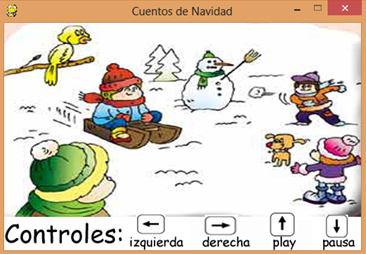
\includegraphics{fo}
\end{center}

\begin{tabular}{lll}

\\Al iniciar la aplicaci\'on solo presentar\'a esta pantalla, en la cual consta de un fondo navide\~no \\
como interfaz del programa y las indicaciones de los controles que permitir\'a al usuario \\
controlar la aplicaci\'on\\



\end{tabular}

\section{Operaci\'on del Programa}

\begin{tabular}{lll}

El cuento iniciar\'a al abrir la aplicaci\'on y llegara al fin de una primera parte, aqui le pedir\'a al\\
usuario que parte del cap\'itulo desea continuar escuchando y para eso se le indicara que \\
cap\'itulo se reproduce al presionar la tecla direccional izquierda  
\includegraphics{iz}y que cap\'itulo se\\
reproduce al presionar la tecla direccional derecha  
\includegraphics{der}.\\
Si en alg\'un momento desea pausar la reproducci\'on de algun cap\'itulo, lo podra hacer pulsando\\
la tecla direccional abajo  
\includegraphics{ab} y para continuar con la reproducci\'on del mismo, lo podra hacer\\
pulsando la tecla direccional arriba  
\includegraphics{arr}.\\
Y para terminar con la aplicaci\'on puede presionar la opci\'on de cerrar en la pantalla o pulsando\\
la tecla ESC.\\


\end{tabular}





\end{document}
